% -----------------------------------------------
% TP1 - Composicao Musical Algoritmica (DCC831, UFMG, 2026/2)
% Resumo no formato ISMIR (template oficial ismir/paper_templates, 2026)
% -----------------------------------------------
\documentclass{article}
\usepackage[T1]{fontenc}
\usepackage[utf8]{inputenc}
\usepackage[submission]{ismir} % remover "submission" na versao final, se desejado
\usepackage{amsmath,cite,url}
\usepackage{graphicx}
\usepackage{color}

\title{Geração de Riffs de Rock 80/90 com Algoritmos Genéticos}

\oneauthor
  {LukasAlbkk}
  {Universidade Federal de Minas Gerais\\Departamento de Ciência da Computação\\\texttt{lucasoom33@gmail.com}}

\def\authorname{L. Albuquerque}

\sloppy

\begin{document}

\maketitle

\begin{abstract}
Este trabalho apresenta um sistema de composição algorítmica que usa um
algoritmo genético (AG) para evoluir riffs de guitarra no estilo rock das
décadas de 1980--90. O genótipo codifica a melodia principal em uma grade
rítmica de colcheias, enquanto o acompanhamento (power chords, baixo e
bateria) é gerado por regras de teoria musical a partir de progressões de
acordes típicas do gênero, fixando a restrição estilística. A função de
fitness combina seis heurísticas (aderência harmônica, suavidade melódica,
densidade rítmica, repetição motívica, cadência e sincopação). O sistema
produz arquivos MIDI e áudio sintetizado reprodutíveis, permitindo gerar
múltiplas músicas a partir da mesma configuração (variando a semente) e ao
variar hiperparâmetros como taxa de mutação, tom, progressão harmônica e
resolução rítmica. Reportamos a evolução do fitness ao longo das gerações
para seis configurações distintas e discutimos os compromissos observados
entre exploração e convergência.
\end{abstract}

\section{Introdução}\label{sec:introduction}

Algoritmos genéticos (AGs) são uma técnica clássica de composição musical
algorítmica: uma população de peças candidatas é avaliada por uma função de
fitness e refinada por seleção, cruzamento e mutação ao longo de gerações
\cite{HornerGoldberg1991}. Este trabalho usa exclusivamente AGs para gerar
riffs de guitarra no estilo \emph{rock} das décadas de 1980 e 1990 --
gênero caracterizado por power chords distorcidos, baixo dobrando a
fundamental, bateria em \emph{backbeat} reto e melodias/riffs pentatônicos
sobre progressões diatônicas simples. Essa restrição estilística orienta
tanto a construção do espaço de busca (alfabeto pentatônico, grade
rítmica) quanto a função de fitness (heurísticas de teoria musical
específicas do idioma do rock).

\section{Trabalhos Relacionados}\label{sec:related}

O uso de AGs em composição musical remonta a
Horner e Goldberg \cite{HornerGoldberg1991}, que evoluíram sequências de
motivos musicais para aproximar uma peça-alvo. Biles \cite{Biles1994GenJam}
propôs o GenJam, um AG interativo que evolui solos de jazz avaliados por um
usuário humano, popularizando fitness interativo em música. Fernández e
Vico \cite{FernandezVico2013} revisam AGs e outras técnicas de IA em
composição algorítmica, situando a escolha de representação e fitness como
os pontos de maior impacto no resultado estético -- decisão central também
neste trabalho, em que optamos por fitness heurístico (regras de teoria
musical) em vez de interativo, por permitir execução em lote e
reprodutibilidade.

\section{Método}\label{sec:method}

\subsection{Representação e restrição estilística}
Cada música tem 16 compassos em 4/4, tom e progressão fixados a partir de
um conjunto curado de progressões típicas do rock 80/90 (p.ex.
i--VI--III--VII, I--V--vi--IV), um acorde por compasso. O acompanhamento
(power chords na guitarra base, baixo na fundamental, bateria com bumbo nos
tempos 1--3 e caixa nos tempos 2--4) é gerado deterministicamente a partir
dessa progressão, fixando o estilo. A saída simbólica é um arquivo MIDI de
4 trilhas; um sintetizador próprio (onda dente-de-serra com harmônicos para
guitarra/baixo e ruído filtrado para bateria) o converte em áudio apenas
para audição.

\subsection{Genótipo}
O AG evolui somente a melodia/riff principal. O genótipo é um vetor de
inteiros de comprimento fixo $L = \text{compassos} \times
\text{passos\_por\_compasso}$ (grade de colcheias, $L=128$ no caso
padrão). Cada gene $\in \{\text{REST}, \text{HOLD}\} \cup \{0..P-1\}$, onde
$P$ é o número de notas da escala pentatônica (menor ou maior, conforme o
tom) disponíveis em cerca de duas oitavas. REST insere silêncio; HOLD
prolonga a nota anterior; um índice de nota inicia uma nova nota. Essa
codificação em grade fixa permite cruzamento e mutação clássicos sem
reparo de genes inválidos.

\subsection{População inicial e função de fitness}
A população inicial ($N{=}80$ indivíduos) é sorteada uniformemente sobre o
alfabeto de genes. O fitness $f \in [0,1]$ é a média ponderada de seis
termos, cada um normalizado em $[0,1]$: (i) \emph{aderência harmônica} --
fração de notas em tempos fortes que são nota do acorde vigente (peso
0.25); (ii) \emph{suavidade melódica} -- recompensa intervalos pequenos
entre notas consecutivas (peso 0.20); (iii) \emph{densidade} -- fração de
passos preenchidos por notas dentro de uma faixa alvo (peso 0.15); (iv)
\emph{repetição motívica} -- similaridade gradual de cada compasso com o
primeiro, incentivando um riff reconhecível (peso 0.15); (v)
\emph{cadência} -- a última nota pertencer ao acorde final (peso 0.10); e
(vi) \emph{sincopação} -- fração de ataques fora do tempo, típica do rock
(peso 0.15).

\subsection{Operadores e critério de parada}
Seleção por torneio ($k{=}3$); cruzamento de um ponto ($p_c{=}0.85$);
mutação por gene ($p_m$, padrão 0.06); elitismo dos 2 melhores indivíduos
por geração. O AG para após 200 gerações ou após 30 gerações sem melhora no
melhor fitness (\emph{early stopping}).

\section{Resultados}\label{sec:results}

Executamos o sistema com seis configurações (Tabela~\ref{tab:runs}): duas
usam a mesma configuração-base variando apenas a semente (song1a/song1b),
demonstrando que músicas distintas emergem da mesma configuração; as
demais variam exatamente um hiperparâmetro em relação à base -- taxa de
mutação, tom/escala/progressão, resolução rítmica (colcheia
vs.\ semicolcheia) e andamento/progressão. A Figura~\ref{fig:single}
mostra a evolução do fitness (melhor, média, pior) para \texttt{song1a};
a Figura~\ref{fig:compare} compara o melhor fitness entre as seis
execuções.

\begin{table}[t]
  \centering
  \small
  \begin{tabular}{|l|l|c|}
    \hline
    \textbf{Execução} & \textbf{Hiperparâmetro variado} & \textbf{Fitness} \\
    \hline
    song1a & (configuração-base) & 0.896 \\
    song1b & semente (mesma config.) & 0.901 \\
    song2 & $p_m$: 0.06 $\to$ 0.20 & 0.755 \\
    song3 & tom maior + prog.\ I-V-vi-IV & 0.861 \\
    song4 & grade de 16{\textordmasculine}s (semicolcheia) & 0.680 \\
    song5 & andamento 96~BPM + prog.\ i-iv-v & 0.940 \\
    \hline
  \end{tabular}
  \caption{Melhor fitness final por execução (ver \texttt{outputs/demo/summary.csv}).}
  \label{tab:runs}
\end{table}

\begin{figure}[t]
  \centering
  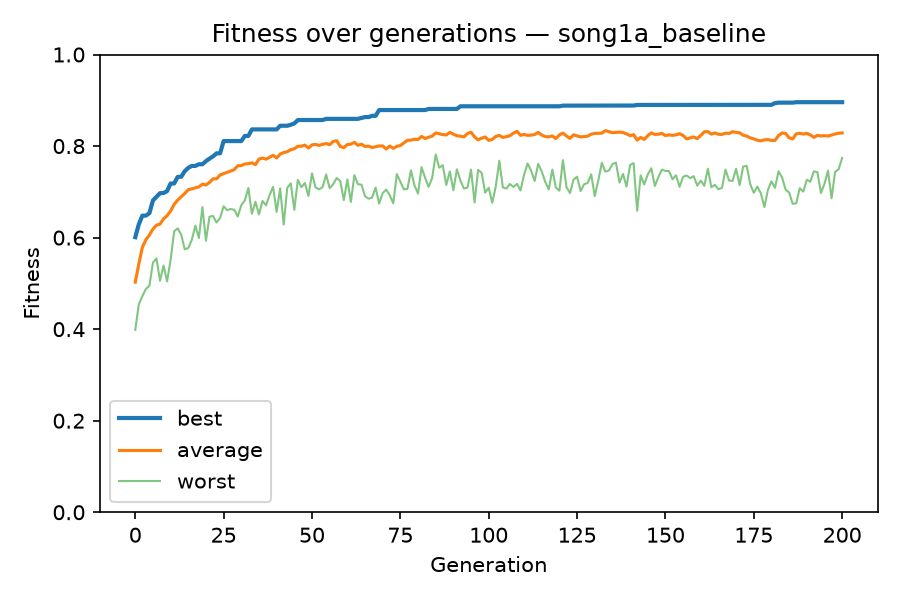
\includegraphics[width=0.95\linewidth]{figures/fitness_song1a.png}
  \caption{Evolução do fitness (melhor/média/pior) -- configuração-base.}
  \label{fig:single}
\end{figure}

\begin{figure}[t]
  \centering
  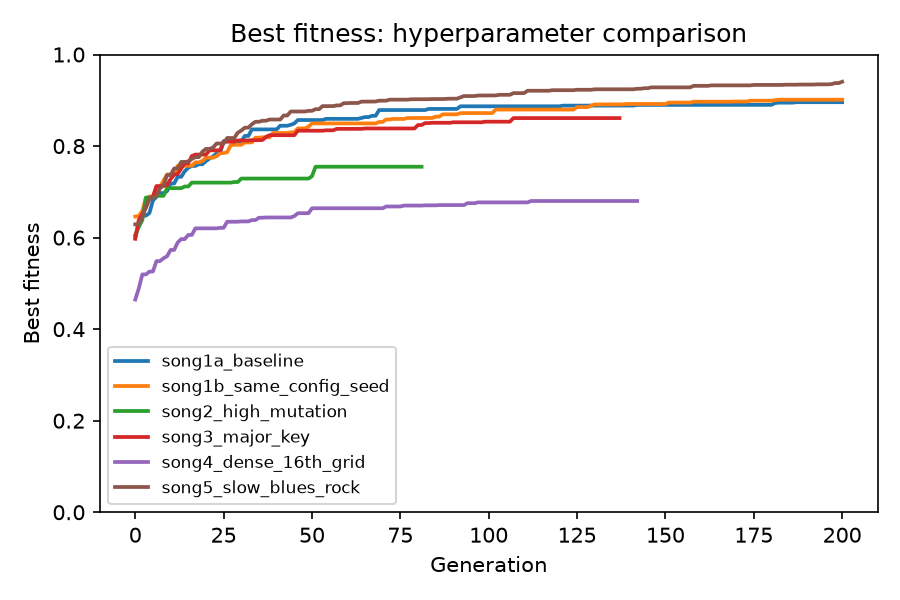
\includegraphics[width=0.95\linewidth]{figures/fitness_comparison.png}
  \caption{Melhor fitness por geração, comparando as seis configurações.}
  \label{fig:compare}
\end{figure}

Qualitativamente, as duas execuções com a mesma configuração (song1a/1b)
convergem para fitness semelhante ($\approx$0.90) mas com riffs
audivelmente distintos, confirmando a variabilidade estocástica do
sistema. Aumentar a taxa de mutação (song2) reduziu o fitness final e
tornou a convergência mais lenta e ruidosa, como esperado ao injetar mais
material aleatório a cada geração. A grade de semicolcheias (song4) tem
espaço de busca maior ($L{=}256$) e obteve o menor fitness dentre as seis
execuções sob o mesmo orçamento de gerações, ilustrando o custo de
resoluções rítmicas mais finas. A configuração mais lenta e com menor
mutação (song5) obteve o maior fitness, favorecida por uma progressão mais
curta (3 acordes) e menor pressão exploratória.

Os seis áudios sintetizados correspondentes (\texttt{outputs/demo/song1a\_baseline.wav}
até \texttt{outputs/demo/song5\_slow\_blues\_rock.wav}), os MIDIs simbólicos
e os logs completos de cada execução estão incluídos no repositório do
projeto.

\section{Discussão e Trabalhos Futuros}\label{sec:discussion}

O fitness heurístico captura bem regras de teoria musical de baixo nível
(aderência harmônica, cadência), mas não avalia originalidade ou
"groove" subjetivo -- um fitness interativo \cite{Biles1994GenJam} poderia
complementar essa limitação ao custo de menor escalabilidade. O
acompanhamento (acordes, baixo, bateria) é fixo por regra, não evoluído;
uma extensão natural é coevoluir múltiplas vozes (ritmo da guitarra base,
variações de bateria) como cromossomos separados ou concatenados, com
operadores de cruzamento que respeitem o alinhamento entre vozes. Também
seria interessante evoluir a própria progressão harmônica dentro de um
conjunto maior de opções, e comparar o fitness heurístico atual com uma
métrica aprendida (p.ex.\ um modelo de linguagem musical) como proxy de
qualidade perceptual.

\bibliography{references}

\end{document}
